\documentclass[tikz,border=20pt]{standalone}
\usepackage{amsmath,amssymb}
\usepackage{tikz}
\usetikzlibrary{matrix, arrows.meta, positioning, fit, backgrounds, calc}

\newcommand{\ideal}[1]{\langle #1\rangle}
\newcommand{\F}{\mathbb F}
\begin{document}
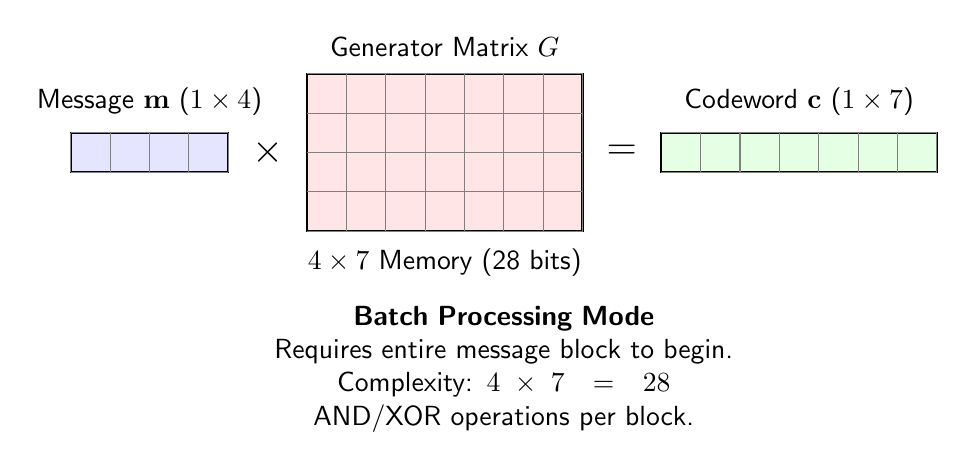
\begin{tikzpicture}[font=\sffamily, >=Stealth]
	
	% 1. Message Vector (1x4)
	\draw[thick, fill=blue!10] (0,0) rectangle (2, 0.5);
	\draw[xstep=0.5cm, ystep=0.5cm, color=black!50] (0,0) grid (2, 0.5);
	\node[above] at (1, 0.6) {Message $\mathbf{m}$ ($1 \times 4$)};
	
	% Multiplication symbol
	\node at (2.5, 0.25) {\Large $\times$};
	
	% 2. Generator Matrix G (4x7)
	% Width = 7 cells * 0.5cm = 3.5cm
	% Height = 4 cells * 0.5cm = 2.0cm
	\draw[thick, fill=red!10] (3, -0.75) rectangle (6.5, 1.25);
	\draw[xstep=0.5cm, ystep=0.5cm, color=black!50, yshift=-.25cm] (3, -0.5) grid (6.5, 1.5);
	\node[above] at (4.75, 1.35) {Generator Matrix $G$};
	\node[below] at (4.75, -0.85) {$4 \times 7$ Memory (28 bits)};
	
	% Equals symbol
	\node at (7, 0.25) {\Large $=$};
	
	% 3. Codeword Vector (1x7)
	% Width = 7 cells * 0.5cm = 3.5cm
	\draw[thick, fill=green!10] (7.5, 0) rectangle (11, 0.5);
	\draw[xstep=0.5cm, ystep=0.5cm, color=black!50] (7.5, 0) grid (11, 0.5);
	\node[above] at (9.25, 0.6) {Codeword $\mathbf{c}$ ($1 \times 7$)};
	
	% 4. Text Annotations comparing complexity
	\node[align=center, text width=8cm] at (5.5, -2.5) {
		\textbf{Batch Processing Mode}\\
		Requires entire message block to begin.\\
		Complexity: $4 \times 7 = 28$ AND/XOR operations per block.
	};
	
\end{tikzpicture}


\vspace{1cm}

% =========================================================
% DIAGRAM 2: LFSR Circuit for Cyclic Code Alternative
% =========================================================
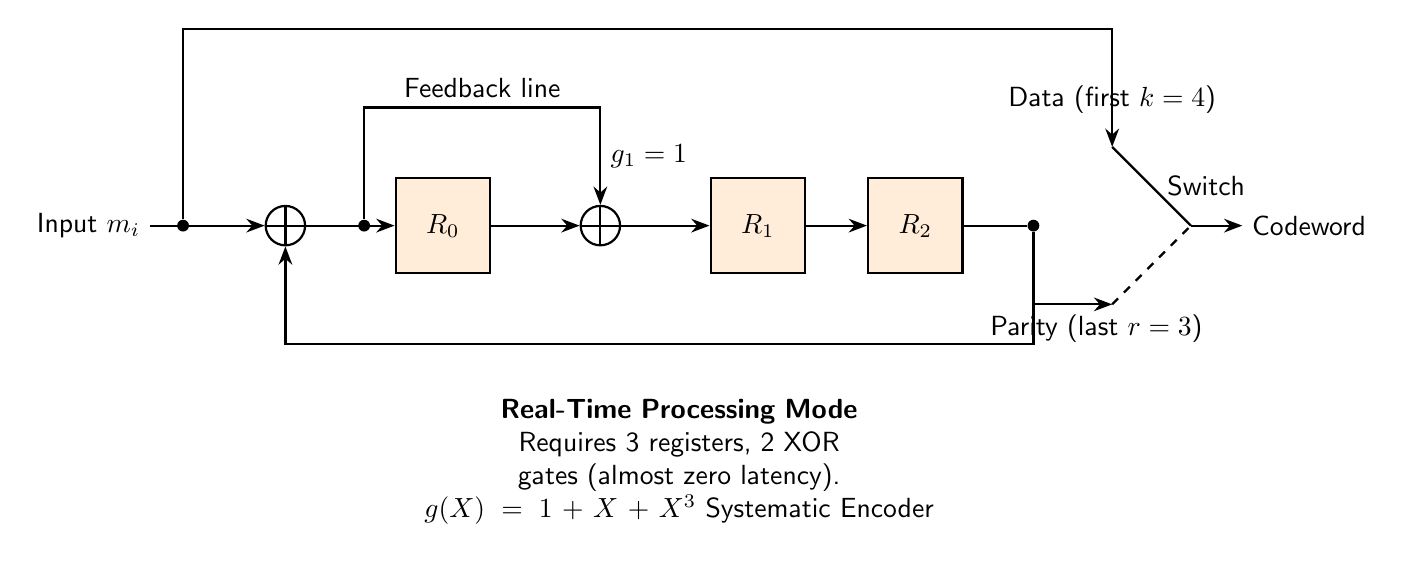
\begin{tikzpicture}[
	font=\sffamily,
	>=Stealth,
	% Style for flip-flop registers
	block/.style={rectangle, draw, minimum width=1.2cm, minimum height=1.2cm, thick, fill=orange!15},
	% Style for XOR gates
	xor/.style={draw, circle, minimum size=0.5cm, thick, fill=white,
		path picture={
			\draw[thick] (path picture bounding box.north) -- (path picture bounding box.south)
			(path picture bounding box.west) -- (path picture bounding box.east);
	}},
	% Style for junction dots
	dot/.style={circle, fill, minimum size=0.15cm, inner sep=0pt}
	]
	
	% 1. Input Node & Split
	\node (msg) at (0,0) {Input $m_i$};
	\node[dot] (msg_split) at (1.2,0) {};
	
	% Feedback XOR gate (combines message and R2 output)
	\node[xor] (xor_in) at (2.5,0) {};
	
	% 2. Shift Registers & Intermediate XORs
	\node[block] (R0) at (4.5,0) {$R_0$};
	\node[xor] (xor1) at (6.5,0) {};
	\node[block] (R1) at (8.5,0) {$R_1$};
	\node[block] (R2) at (10.5,0) {$R_2$};
	
	% 3. Output tap for Feedback & Parity
	\node[dot] (R2_split) at (12,0) {};
	
	% 4. Draw Main Datapath (Horizontal)
	\draw[thick, ->] (msg) -- (xor_in);
	\draw[thick, ->] (xor_in) -- (R0);
	\draw[thick, ->] (R0) -- (xor1);
	\draw[thick, ->] (xor1) -- (R1);
	\draw[thick, ->] (R1) -- (R2);
	\draw[thick, -]  (R2) -- (R2_split);
	
	% 5. Top Feedback Line (F) for generator coefficients
	\node[dot] (F_split) at (3.5,0) {};
	% Line goes up, across to g_1, and drops into xor1
	\draw[thick, ->] (F_split) -- (3.5, 1.5) -- (6.5, 1.5) -- (xor1) 
	node[midway, right] {$g_1=1$};
	\node[above] at (5, 1.5) {Feedback line};
	
	% 6. Bottom Return Line (from R2 back to input XOR)
	% This represents g_3 = 1
	\draw[thick, ->] (R2_split) -- (12, -1.5) -- (2.5, -1.5) -- (xor_in);
	
	% 7. Output Switch Setup
	\coordinate (sw_msg) at (13, 1);
	\coordinate (sw_parity) at (13, -1);
	\coordinate (sw_out) at (14, 0);
	\node (codeword) at (15.5, 0) {Codeword};
	
	% Path routing raw message to the top of the switch
	\draw[thick, ->] (msg_split) -- (1.2, 2.5) -- (13, 2.5) -- (sw_msg) 
	node[above, pos=0.8] {Data (first $k=4$)};
	
	% Path routing parity bits to the bottom of the switch
	\draw[thick, ->] (R2_split) -- (12, -1) -- (sw_parity) 
	node[below, pos=0.8] {Parity (last $r=3$)};
	
	% Draw the physical switch
	\draw[thick, -] (sw_msg) -- (sw_out) node[midway, right=2pt] {Switch};
	\draw[thick, dashed, -] (sw_parity) -- (sw_out); % Shows alternate position
	\draw[thick, ->] (sw_out) -- (codeword);
	
	% 8. Text Annotations
	\node[align=center, text width=8cm] at (7.5, -3) {
		\textbf{Real-Time Processing Mode}\\
		Requires 3 registers, 2 XOR gates (almost zero latency).\\
		$g(X) = 1 + X + X^3$ Systematic Encoder
	};
	
\end{tikzpicture}
\end{document}